\documentclass[11pt]{article}
\usepackage{geometry} % Pour passer au format A4
\geometry{hmargin=1cm, vmargin=1cm} % 

% Page et encodage
\usepackage[T1]{fontenc} % Use 8-bit encoding that has 256 glyphs
\usepackage[english,francais]{babel} % Français et anglais
\usepackage[utf8]{inputenc} 

\usepackage{lmodern}
\setlength\parindent{0pt}

% Graphiques
\usepackage{graphicx, float}


% Maths et divers
\usepackage{amsmath,amsfonts,amssymb,amsthm,verbatim}
\usepackage{multicol,enumitem,url,eurosym,gensymb}

% Sections
\usepackage{sectsty} % Allows customizing section commands
\allsectionsfont{\centering \normalfont\scshape}

% Tête et pied de page

\usepackage{fancyhdr} 
\pagestyle{fancyplain} 

\fancyhead{} % No page header
\fancyfoot{}

\renewcommand{\headrulewidth}{0pt} % Remove header underlines
\renewcommand{\footrulewidth}{0pt} % Remove footer underlines

\newcommand{\horrule}[1]{\rule{\linewidth}{#1}} % Create horizontal rule command with 1 argument of height

%----------------------------------------------------------------------------------------
%	Début du document
%----------------------------------------------------------------------------------------

\begin{document}

\textbf{Nom, Prénom :} \hspace{8cm} \textbf{Classe :} \hspace{3cm} \textbf{Date :}\\


\begin{center}
  \textit{Les mathématiques ne sont une moindre immensité que la mer.}  - \textbf{Victor Hugo}
\end{center}

\textit{La présentation, la rédaction et le soin général apportés à la copie sont sur 3 points.}
\begin{itemize}
\item \textsc{Calculer} : 
\item \textsc{Modéliser} : 
\item \textsc{Note} : 
\end{itemize}

\horrule{1px}
\vspace{-1cm}

\subsubsection*{Modéliser}
Parmi les situations suivantes, trouve celles dont les deux triangles sont en situation
pour pouvoir utiliser le théorème de Thalès. Si les triangles sont en situation pour pouvoir utiliser le théorème de Thalès, donne
l’égalité des trois rapports.
On donne : (IJ) // (GH) ; et (FG) // (HI).

\begin{figure}[H]
  \centering
  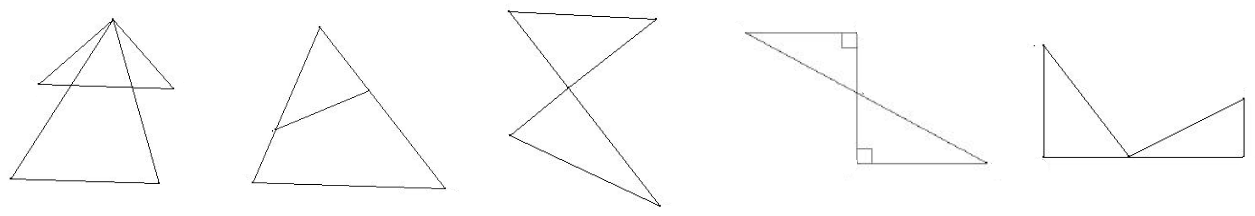
\includegraphics[width=0.8\linewidth]{sources/ch5-thales/1_modele.png}
\end{figure}

\subsubsection*{Calculer}

Calculer les longueurs indiquées. On donne (NP) // (RS) ; (MN) // (BC) et (BC) // (MN)

\begin{figure}[H]
  \centering
  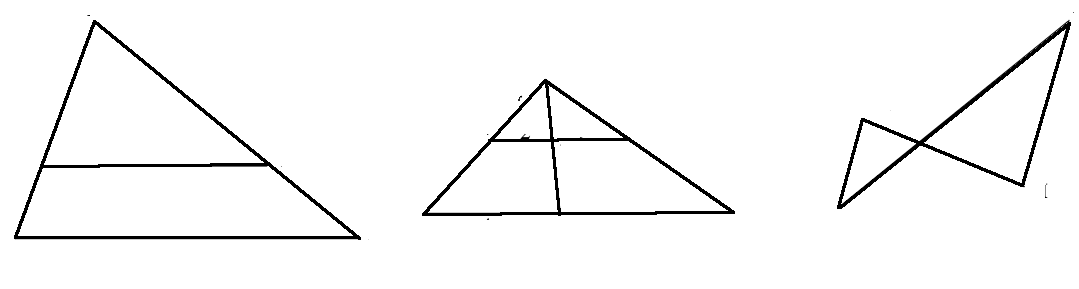
\includegraphics[width=0.8\linewidth]{sources/ch5-thales/2_longueurs.png}
\end{figure}



\begin{multicols}{2}

\subsubsection*{Problème 1 - Voiture}

Pour effectuer un réglage rapide des feux de croisement d'un vehicule, on place celui-ci devant un mur vertical. La portée des feux est HM = 40m. La hauteur des feux est HP = 0.8m. La distance entre la voiture et le mur est AH = 4m.

\begin{enumerate}
  \item[1a.] Calculer AM.
  \item[1b.] Calculer la hauteur de réglage AB.
\end{enumerate}

\begin{figure}[H]
  \centering
  \includegraphics[width=0.6\linewidth]{sources/ch5-thales/pb1.pdf}
\end{figure}

\end{multicols}

\begin{multicols}{2}

\subsubsection*{Problème 2 - Bateau}

On souhaite construire une voile pour un bateau. On doit coudre le segment [CT] sur la voile. On donne : PC = 3.78m, PM = 4.20m et MW = 3.40m.

\begin{enumerate}
  \item[2a.] Estimation. On suppose (CT) // (MW). La quantité de fil nécéssaire est le triple de la couture. Quelle est la longueur du fil nécessaire à la couture ?
\end{enumerate}

\begin{figure}[H]
  \centering
  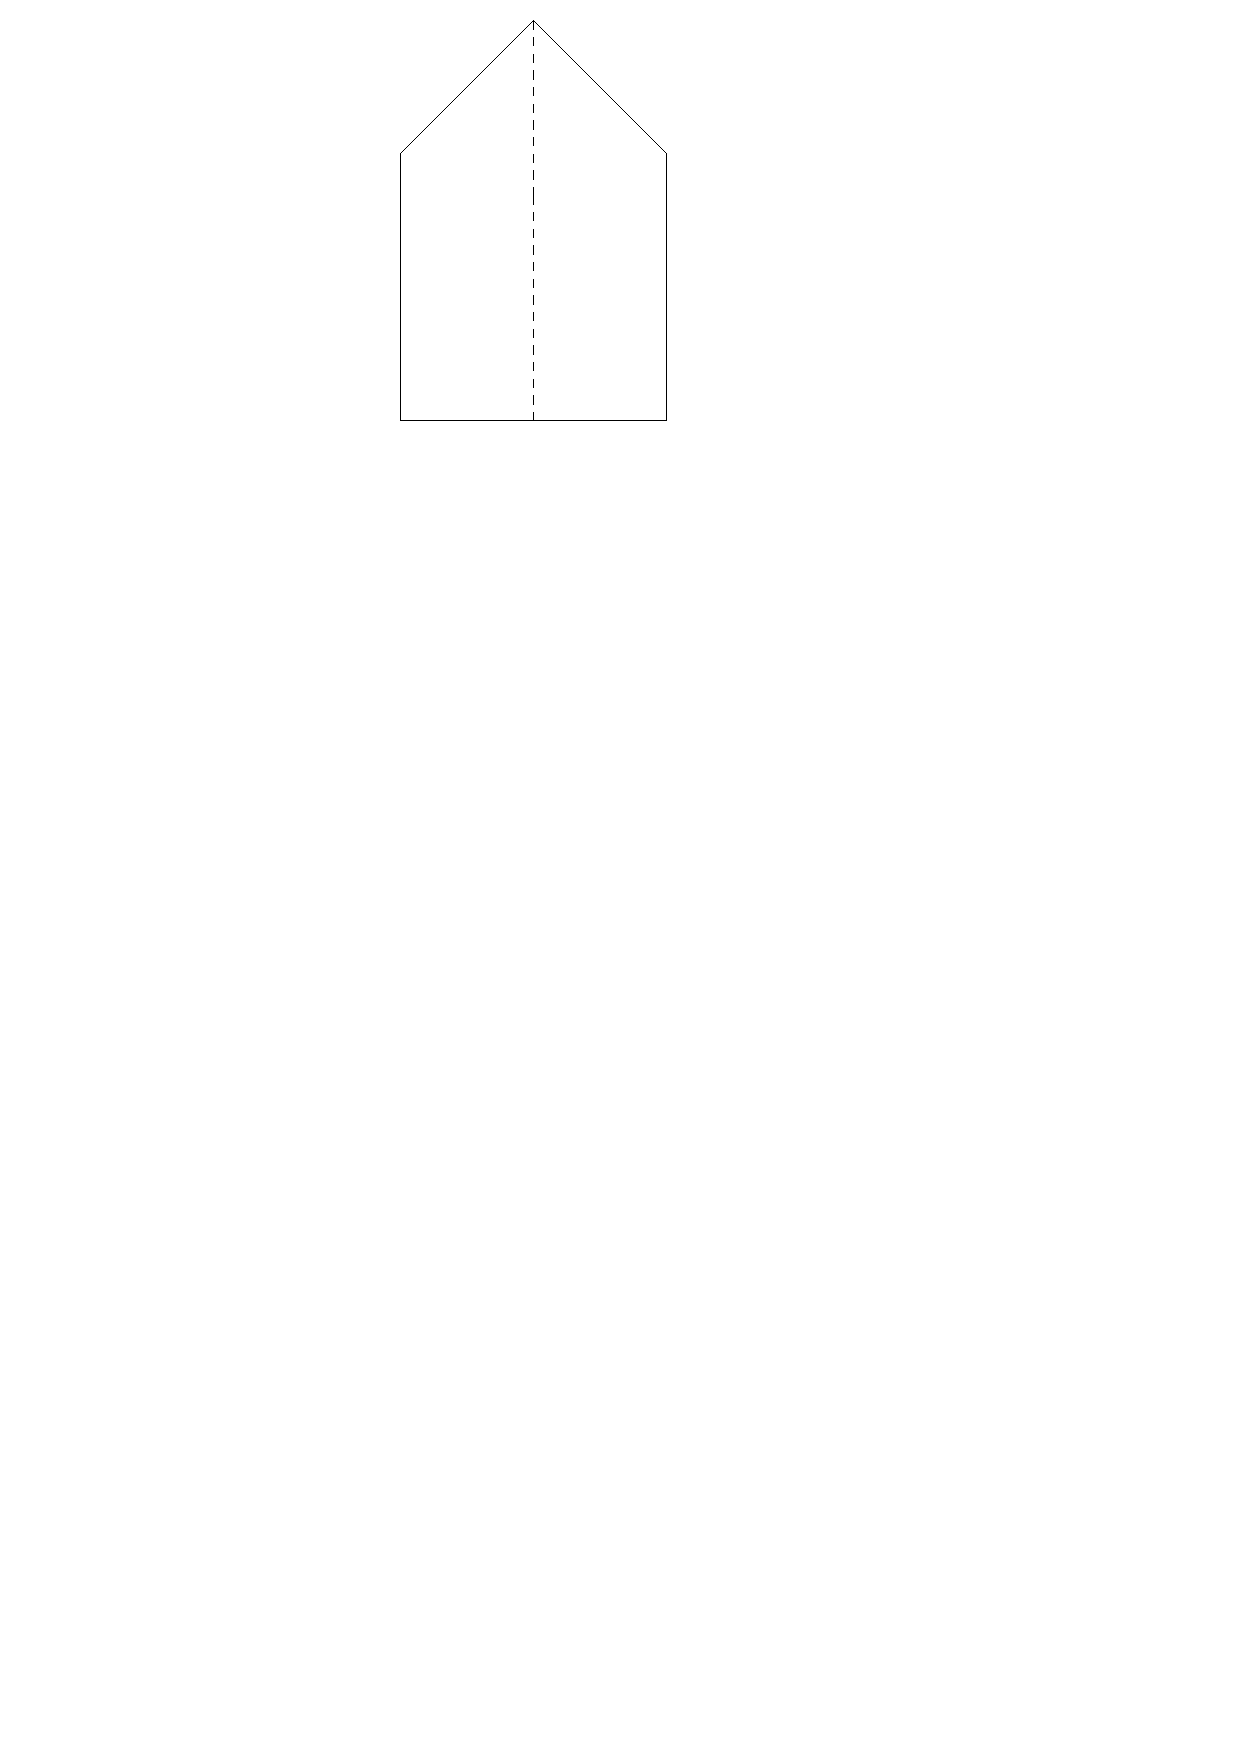
\includegraphics[width=0.5\linewidth]{sources/ch5-thales/pb2.pdf}
\end{figure}

\end{multicols}

\end{document}
